
% Experement data + calcs goes here %

\section{Ход работы}

\subsection{Сравнение теоретического и измеренного периодов колебаний}

Период, снятый с осциллографа: \mth{T\ruB{изм} = (34,0\pm0,3)10^{-5}}c \\ [0.2cm]

\noindentТеоретический период, расчитанный через L и C: \mth{T\ruB{теор} = (33,4\pm0,6)10^{-5}}c \\ [0.2cm]

\noindentВидно, что в пределах погрешности, данные величины совпадают. \\ [0.2cm]

\subsection{Измерение логарифмического декремента и добротности контура}

Наблюдая за затуханием колебаний в контуре при разных сопротивлениях \mth{R}, и зная, что зависимость \mth{R(\Theta)} линейна, найдем для LC контура его сопротивление и логарифмический декремент затухания. 

\begin{center}

    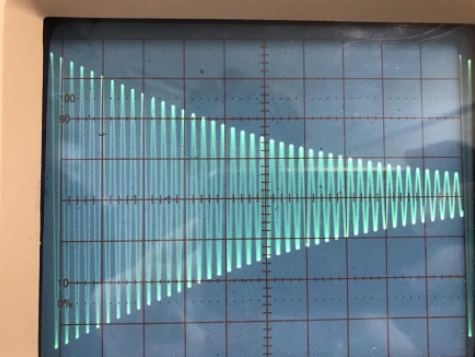
\includegraphics[scale=0.9]{324-oscl1.png} \\
    \textit{Рис. 2. Затухания в контуре}

\end{center}

Данные представлены в таблице 1:


\begin{table}[!h]
    \begin{center}
    \begin{tabular}{|c|c|c|c|c|}
    \hline
    R, Ом & n  & \mth{U_k}, дел & \mth{U_{k+n}}, дел & \mth{\Theta, 10^{-2}} \\ \hline
    0     & 22 &     4      &        2        &        3,151      \\ \hline
    2     & 21 &     4      &        2        &        3,301      \\ \hline
    4     & 20 &     4      &        2        &        3,466      \\ \hline
    6     & 19 &     4      &        2        &        3,648      \\ \hline
    8     & 18 &     4      &        2        &        3,851      \\ \hline
    10    & 17 &     4      &        2        &        4,077      \\ \hline
    12    & 16 &     4      &        2        &        4,332      \\ \hline
    14    & 15 &     4      &        2        &        4,621      \\ \hline
    \end{tabular} \\ [0.2cm]
    \textit{Таблица 1. Данные.}
    \end{center}
\end{table}
\newpage

По методу наименьших квадратов построю график линейной зависимости \mth{R(\Theta)}:

\begin{center}

    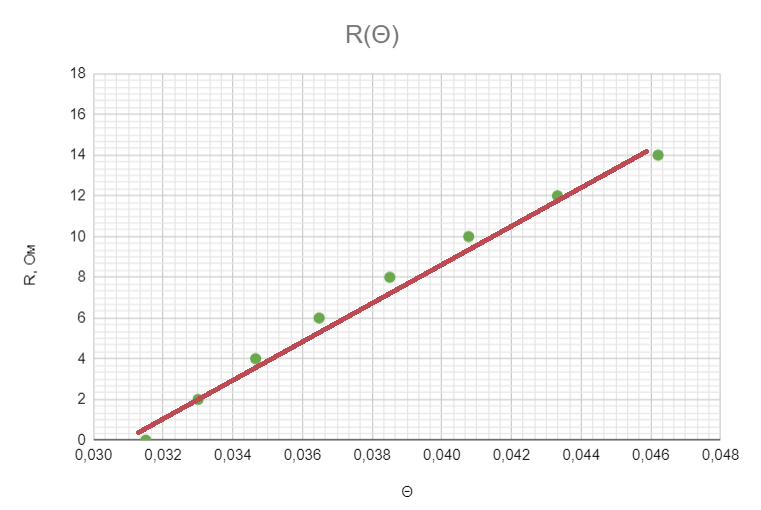
\includegraphics[scale=0.9]{324-R-th.png} \\
    \textit{Рис. 4. Зависимость \mth{R(\Theta)}}

\end{center}

\noindentИз к-та b найду сопротивление LC контура: \mth{R_0 = 36,1 \pm 2,1} Ом. \\ [0.2cm]

\noindentИз к-та наклона найду критическое сопротивление LC контура: \mth{R\ruB{кр.} = 8000 \pm 400} Ом. \\ [0.2cm]

\noindentПодобрал значение критического сопротивления путем увеличения сопротивления до тех пор, пока на экране осциллографа не исчезнут колебания: \mth{R\ruB{кр. подб.} \approx 7600} Ом. \\ [0.2cm]

\begin{center}

    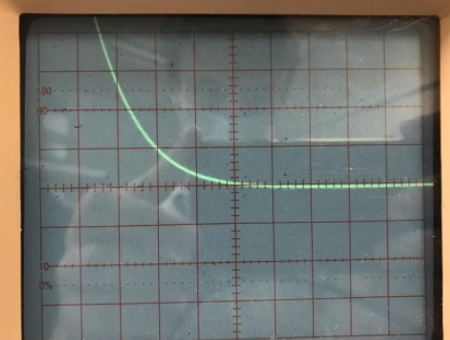
\includegraphics[scale=0.9]{324-oscl2.png} \\
    \textit{Рис. 5. График без колебаний}

\end{center}

Видно, что полученные значения для критического сопротивления LC цепи совпадают в пределах погрешности.

\newpage

\subsection{Определение добротности}

Определею добротность контура с помощью данных таблицы 1 и сравню результат с расчетом через R, L и С. Результаты расчетов представлены в таблице 2.

\begin{table}[!h]
    \begin{center}
    \begin{tabular}{|c|c|c|c|}
    \hline
    R, Ом & Q(R)   & \mth{\Theta} &  Q(\mth{\Theta}) \\ \hline
    36,09 & 101,46 &     0,032    &       99,71      \\ \hline
    38,09 & 96,27  &     0,033    &       95,18      \\ \hline
    40,09 & 91,58  &     0,035    &       90,65      \\ \hline
    42,09 & 87,33  &     0,036    &       86,11      \\ \hline
    44,09 & 81,65  &     0,039    &       81,58      \\ \hline
    46,09 & 78,25  &     0,041    &       77,05      \\ \hline
    48,09 & 75,13  &     0,043    &       72,52      \\ \hline
    50,09 & 72,24  &     0,046    &       67,99      \\ \hline
    \end{tabular} \\ [0.2cm]
    \textit{Таблица 2. Добротность.}
    \end{center}
\end{table}

\noindentВидно, что результаты расчетов сходятся в пределах погрешностей.

\subsection{Определение логарифмического декремента затухания по X-Y диаграмме}

Если перевести переключатель TIMES-DIV в положение X-Y, то можно получить следующую картину:

\begin{center}

    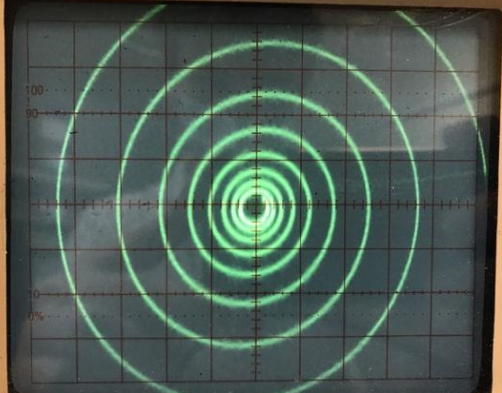
\includegraphics[scale=0.9]{324-oscl3.png} \\
    \textit{Рис. 6. X-Y диаграмма}

\end{center}

\noindentПо данной диаграмме можно определить логарифмический декремент затухания и сравнить его с теоретическим значением, полученным через R, L и C.

\newpage

\subsubsection{Для R = 800 Ом}
\mth{X_k = 3,6} дел. \mth{X_{k + n} = 2,8} дел. Тогда \mth{\Theta = 0,687}. \\ [0.2cm]
Значение полученное по формуле: \mth{\Theta\ruB{теор} = 0,663}.

\subsubsection{Для R = 400 Ом}
\mth{X_k = 2,5} дел. \mth{X_{k + n} = 1,2} дел. Тогда \mth{\Theta = 0,331}.
Значение полученное по формуле: \mth{\Theta\ruB{теор} = 0,332}. \\ [0.2cm]

\noindentВидно, что данные значения сходятся в пределах погрешности.

\section{Заключение}

В ходе выполнения лабараторной работы все полученные значения: индуктивности, логарифмического декремента затухания, добротности, совпали с теоретическими расчетами. Также был получен линейный график для зависимости R(\mth{\Theta}), что также согласуется с теорией. \\ [0.3cm]

\noindentОМ БЫЛ ПРАВ. f